\documentclass[tikz]{standalone}

\usepackage{amsmath}
\usepackage{unicode-math}
\usepackage{mathtools}
\usepackage{derivative}

\setmainfont{Stix Two Text}
\setmathfont{Stix Two Math}

\usetikzlibrary{arrows.meta,fit,positioning}

\renewcommand{\familydefault}{\sfdefault}

% prefix equation numbers with section number
\numberwithin{equation}{section}

\DeclarePairedDelimiter{\ceil}{\lceil}{\rceil}
\DeclarePairedDelimiter{\floor}{\lfloor}{\rfloor}
\DeclarePairedDelimiter{\abs}{\lvert}{\rvert}
\DeclarePairedDelimiter{\norm}{\lVert}{\rVert}
\DeclarePairedDelimiter{\bra}{\langle}{\rvert}
\DeclarePairedDelimiter{\ket}{\lvert}{\rangle}
\DeclarePairedDelimiter{\expval}{\langle}{\rangle}
\DeclarePairedDelimiter{\norder}{\mathcolon}{\mathcolon}
\DeclarePairedDelimiter{\anorder}{\typecolon}{\typecolon}
	
\newcommand{\laplace}{\mbfnabla^2}
\newcommand{\trans}{{\scriptscriptstyle\mathsf{T}}}

\newcommand{\vdot}{\cdot}
\newcommand{\vcross}{\vectimes}
\newcommand{\vb}[1]{\symbfup{#1}}
\newcommand{\vu}[1]{\hat{\vb{#1}}}
\newcommand*\dd[2][\relax]{\mathop{\ifx\relax#1\odif{#2}\else \odif[order={#1}]{#2}\fi\,}}

\newcommand{\vacuum}{\ket*{\vb{0}}}

\DeclareMathOperator{\trace}{Tr}
\DeclareMathOperator{\sinc}{sinc}

\AtBeginDocument{
	\let\Re\relax
	\let\Im\relax
	\DeclareMathOperator{\Re}{Re}
	\DeclareMathOperator{\Im}{Im}

	\renewcommand{\div}{\mathop{\mbfnabla\vdot}}
	\newcommand{\curl}{\mathop{\mbfnabla\vectimes}}
}

\DeclarePairedDelimiterX{\comm}[2]{[}{]}{#1,#2}

\DeclarePairedDelimiterX{\braket}[2]{\langle}{\rangle}{#1\delimsize\vert#2}
\DeclarePairedDelimiterX{\ketbra}[1]{\lvert}{\rvert}{#1\rangle\delimsize\langle#1}



\begin{document}
    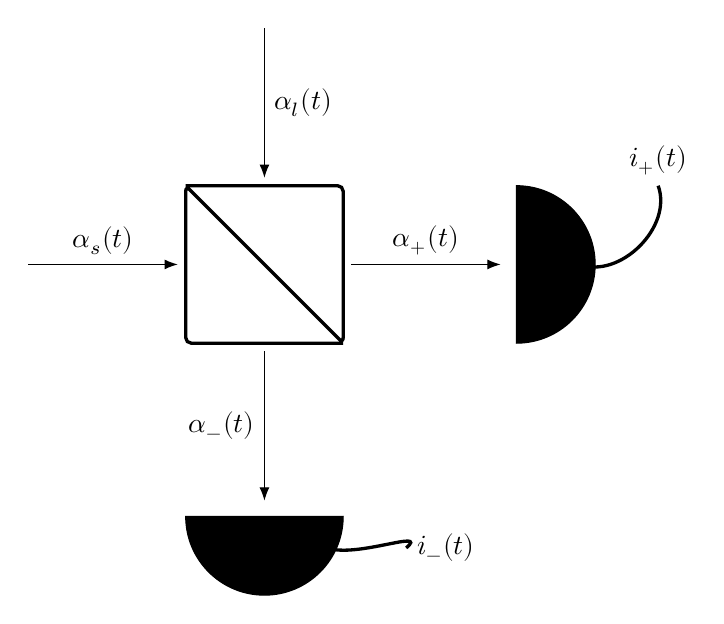
\begin{tikzpicture}
        \draw[very thick, rounded corners=2pt] (0, 0) -- ++(2, 0) -- ++(0, -2) -- (0, 0) -- ++(0, -2) -- ++(2, 0);
        
        \draw[fill, rotate=-90, yshift=22mm] (2, 2) -- (2, 2) arc(0:180:1) --cycle;
        \draw[fill=black, rotate=-180, yshift=22mm, xshift=-20mm] (2, 2) -- (2, 2) arc(0:180:1) --cycle;
   
        \draw[very thick] (5, -1) to[out=-20, in=-70] ++(1, 1) node[above] {$i_+(t)$};
        \draw[very thick] (1.8, -4.6) to[out=-20, in=40] ++(1, 0) node[right] {$i_-(t)$};
        
        \draw[-Latex] (-2, -1) -- ++(1.9, 0) node[midway, above] {$\alpha_s(t)$};
        \draw[-Latex] (1, 2) -- ++(0, -1.9) node[midway, right] {$\alpha_l(t)$};
        \draw[Latex-] (1, -4) -- ++(0, 1.9) node[midway, left] {$\alpha_-(t)$};
        \draw[Latex-] (4, -1) -- ++(-1.9, 0) node[midway, above] {$\alpha_+(t)$};
    \end{tikzpicture}
\end{document}
